\chapter{Implementacja}
\thispagestyle{chapterBeginStyle}

Implementacja $\mathbf{RiffleScrambler}$ została napisana tak, aby spełniała wymagania konkursu na funkcję do przechowywania haseł \cite[PHC, ang \textit{Password Hashing Competition}]{PHC2013}, który rozgrywał się w latach 2013 - 2015.

\section{Wymagania konkursu}
Wymagania konkursu PHC odnoszące się do implementacji:
\begin{itemize}
	\item implementacja powinna być napisana w języku C(++) w taki sposób, aby była przenośna,
	\item do implementacji powinny być dołączone instrukcje kompilacji (np. Makefile),
	\item interfejs powinien być dostępny do użycia w języku C, oraz powinien zapewniać funkcję z podaną poniżej sygnaturą \ref{impl::phc},
	\item implementacja może używać biblioteki OpenSSL,
	\item do implementacji powinny zostać dołączone testy.
\end{itemize}

\begin{minted}[mathescape]{C}
// Interfejs zaproponowany w ogłoszeniu konkursu na funkcję do przechowywania haseł $\cite{PHC2013}$ $\label{impl::phc}$
int PHS(void *out, size_t outlen, const void *in, size_t inlen,
	const void *salt, size_t saltlen, % unsigned int t_cost, unsigned int m_cost); 
\end{minted}

Na zwycięzce konkursu wybrano Argon2, a Catena, Lyra2, yescryot oraz Makwa otrzymały specjalne wyróżnienie.

\section{Opis technologii}
Początkowa implementacja napisana została w języku Python 3.7, jednak ze względu na niską wydajność oraz nie spełnianie wymagań PHC napisana została ostatecznie w języku C++17, standard ISO/IEC 14882:2017.

W implementacji używana jest biblioteka OpenSSL w wersji ...,
Z podanej biblioteki użyto interfejsu EVP który dostarcza podstawowe kryptograficzne funkcje skrótu takie jak SHA2, SHA3, blake2s czy ripemd160.


\section{Omówienie kodów źródłowych}
Omówiony zostanie interfejs funkcji $\mathbf{RiffleScrambler}$, który spełnia wymogi PHC oraz posiada dodatkowy wysokopoziomowy interfejs pozwalający na wygodne tworzenie aplikacji uwierzytelniającej.

Kompletne kody źródłowe znajdują się do płycie CD dołączonej do niniejszej pracy. (patrz Dodatek A).

\subsection{Wysokopoziomowy interfejs}
Wysokopoziomowy interfejs upraszcza użycie funkcji $\mathbf{RiffleScrambler}$ podczas pisania
programów na wyższym abstrakcji takich jak na przykład aplikacje uwierzytelniające.
Podobnie jak w implementacji zwycięzcy konkursu PHC (argon2 \cite{Argon2}) w udostępnionych funkcjach znajdują się:
\begin{itemize}
	\item funkcja zwracająca wynik jako tekst ze znakami w systemie heksadecymalnym - linia \ref{impl::rs_str},
	\item funkcja zwracająca wynik jako wektor znaków w systemie heksadecymalnym - linia \ref{impl::rs_vec},
	\item funkcja zwracająca zakodowany wynik wraz z użytą solą oraz parametrami w celu łatwego przechowywania i łatwej weryfikacji, sól oraz hasło zakodowane są za pomocą base64 \cite{base64} - linia \ref{impl::rs_enc},
	\item funkcja weryfikująca poprawność podanego hasła dla zakodowanego wyniku - linia \ref{impl::rs_ver}.
\end{itemize}

Każda z podanych funkcji ma również sygnaturę, gdzie hasło i sól podawane są za pomocą typu \texttt{std::string}.

\begin{minted}[linenos=true, mathescape]{C++}

/**$\label{impl::rs_str}$
* Hashowanie hasła za pomocą RiffleScrambler 
* @param pwd Wskaźnik na hasło
* @param pwdlen_bytes Długość hasła w bajtach
* @param salt Wskaźnik na sól
* @param saltlen_bytes Długość soli w bajtach
* @param garlic Paremetr "g" oznaczający koszt pamięci
* @param depth Parametr "lambda" oznaczający koszt czasowy
* @param hash_func Nazwa kryptograficznej funkcji skrótu do użycia wewnątrz
* @return Hash hasła jako ciąg znaków w systemie szesnastkowym
*/
std::string riffle_scrambler(const void *const pwd, const size_t pwdlen_bytes,
const void *const salt, const size_t saltlen_bytes,
const uint64_t garlic, const uint64_t depth,
const std::string hash_func="sha256");


/** $\label{impl::rs_vec}$
* Hashowanie hasła za pomocą RiffleScrambler
* @param garlic Paremetr "g" oznaczający koszt pamięci
* @param depth Parametr "lambda" oznaczający koszt czasowy
* @param pwd Wskaźnik na hasło
* @param pwdlen_bytes Długość hasła w bajtach
* @param salt Wskaźnik na sól
* @param saltlen_bytes Długość soli w bajtach
* @param hash_func Nazwa kryptograficznej funkcji skrótu do użycia wewnątrz
* @return Hash hasła jako wektor znaków w systemie szesnastkowym
*/
std::vector<unsigned char> riffle_scrambler_hash_raw(const uint64_t garlic,
const uint64_t depth, const void *pwd, const size_t pwdlen_bytes,
const void *salt, const size_t saltlen_bytes, const std::string hash_func="sha256");


/**$\label{impl::rs_enc}$
* Hashowanie hasła za pomocą RiffleScrambler  
* kodowanie wyniku wraz z parametrami w jeden ciąg znaków
* @param garlic Paremetr "g" oznaczający koszt pamięci
* @param depth Parametr "lambda" oznaczający koszt czasowy
* @param pwd Wskaźnik na hasło
* @param pwdlen_bytes Długość hasła w bajtach
* @param salt Wskaźnik na sól
* @param saltlen_bytes Długość soli w bajtach
* @param hash_func Nazwa kryptograficznej funkcji skrótu do użycia wewnątrz
* @return Zakodowane parametry funkcji wraz z hashem hasła i solą
*/
std::string riffle_scrambler_encoded(const uint64_t garlic, const uint64_t depth,
const void *pwd, const size_t pwdlen_bytes,
const void *salt, const size_t saltlen_bytes, const std::string hash_func="sha256");


/** $\label{impl::rs_ver}$
* Weryfikacja hasha hasła z hashem zakodowanym hashem dla zakodowanych parametrów i soli
* @param encoded Zakodowane parametry wraz z hashem i solą
* @param pwd Wskaźnik na hasło
* @param pwd_len Długość hasła w bajtach
* @return true jeśli hashe są równe, false w przeciwny przypadku
*/
bool riffle_scrambler_verify(const std::string encoded, const void *pwd, const size_t pwd_len);


\end{minted}

\subsection{Niskopoziomowy interfejs}
Implementacja jest zgodna z interfejsem zaproponowanym przez PHC.
\begin{minted}[linenos=true, mathescape]{C++}
/**
* Hashowanie hasła za pomocą RiffleScrambler, wynik zwracany jest do zmiennej @hash
* @param pwd Wskaźnik na hasło
* @param pwdlen_bytes Rozmiar hasła w bajtach
* @param salt Wskaźnika na sól
* @param saltlen_bytes Rozmiar soli w bajtach
* @param t_cost Parametr "lambda" oznaczający ilość iteracji
* @param m_cost Parametr "g" oznaczający koszt rozmiar używanej pamięci
* @param hash Bufor do którego będzie zapisany hash hasła
* @param hashlen Rozmiar bufora, oznacza ile bajtów z hasha hasła ma zostać zapisane
* @return RIFFLE_SCRAMBLER_OK jeśli obliczenia zakończyły się pomyślnie, kod błędu w przeciwnym przypadku
*/
int riffle_scrambler(void *hash, const size_t hashlen, const void *pwd, const size_t pwdlen_bytes,
const void *salt, const size_t saltlen_bytes, const uint64_t t_cost, const uint64_t m_cost);
\end{minted}


\section{Parametry}
Funkcja przyjmuje parametry opisane w poprzednim rozdziale [\nameref{rs::g}].
\begin{itemize}
	\item Parametr \texttt{garlic} oznacza $g$ z poprzedniego rozdziału, czyli długość rzędu, która wynosi $N = 2^{g}$.
	Definiuje to rozmiar pamięci, która jest potrzebny do wykonania obliczeń.
	Ponieważ w pamięci trzymane są wartości z dwóch rzędów grafu w jednej chwili, czyli dwóch rzędów po $2^g$ elementów, gdzie każda trzyma wynik wewnętrznej funkcji haszującej. Zatem zapotrzebowanie na pamięć wynosi $2^{g + 1} \times m$, gdzie $m$ oznacza rozmiar wyniku funkcji haszującej (np. dla SHA256 jest to 256 bitów, tak jak wskazuje nazwa).
	Na ogólne zużycie pamięci przez program w obecnej wersji wpływa też graf, który jest generowany na początku i trzymany przez czas działania programu. Przyjmuje wartość od $0$ do $2^{24} - 1$.
	
	\item Parametr \texttt{depth} oznacza ilość warstw grafu i w poprzednim rozdziale oznaczony był jako $\lambda$, przyjmuje wartość całkowitą od $1$ do $2^{64} - 1$.
	
	\item \texttt{pwd} oznacza hasło. Może być to wskaźnik na dane o długości od $0$ do $2^{32} -1$ bitów. Nie jest sprawdzana jakość hasła.
	Zapewnienie, że podane hasło jest wystarczające długie lub spełnia pewne warunki leży po stronie programu używającego funkcję $\mathbf{RiffleScrambler}$.
	\item Parametr \texttt{salt} dostarcza do programu sól kryptograficzną o długości od $0$ do $2^{32} - 1$ bitów. Powinna być ona losowa oraz inna dla każdego z przechowywanych haseł, zalecaną długością soli jest co najmniej 16 bajtów \cite{PHC2013}.
	
	\item Parametr \texttt{hash\_func} określa funkcję hashującą, która ma być użyta wewnątrz $\mathbf{RiffleScrambler}$. Dostępne są następujące funkcje: sha224, sha256, sha384, sha512, ripemd160, blake2s256, blake2s512 oraz do celów testowych sha1, md5, mdc2.
\end{itemize}

Ważny jest dobór parametrów \texttt{garlic} ($g$) oraz \texttt{depth} ($\lambda$), ponieważ to od nich zależy bezpieczeństwo przechowywanych haseł. Zalecanymi parametrami, podobnie jak dla Argon2, jest $\texttt{garlic}=12$ oraz $\texttt{depth}=4$ zapewniające dostateczne bezpieczeństwo oraz racjonalny czas obliczeń. Oznacza to użycie pamięci wynoszące $16$ MiB, co jest wyższą wartością niż rozmiar pamięci podręcznej na poziomie L-1 oraz L-2 dla większości procesorów, a zazwyczaj nawet większa od całkowitej pamięci podręcznej, co wymusza kosztowne sięganie do pamięci RAM. 

\section{Uwidacznianie się własności \textit{memory-hard}}
Implementacja została zbadana pod kontem wydajności w zależności od podawanych parametrów.
Na podstawie wyników można zaobserwować, jak uwidacznia się własność \textit{memory-hard}.

Na wykresie \ref{impl::b2} widać, że zużycie pamięci rośnie wykładniczo od wartości parametru $g$.
Ponieważ zapotrzebowanie na pamięć rośnie, procentowo mniej elementów mieści się w pamięci podręcznej.

Dobrze odwzorowuje to wykres \ref{impl::b1}. Oprócz sytuacji dla $g < 7$, którą ciężko wyjaśnić, a więc biorąc pod uwagę wartości dla $g \geq 7$, liczba odwołań do danych, które nie znajdowały się w pamięci podręcznej (ang. \textit{chache misses}) zaczyna rosnąć od pewnego momentu.
Pierwszy wzrost ma miejsce dla $g = 10$, co odpowiada zapotrzebowaniu na pamięć ok. $1$ MiB. Biorąc pod uwagę, że pamięć podręczna obsługuje również inne procesy, w tym program monitorujący, można wnioskować, że liczba odczytów z pamięci RAM zaczyna być procentowo coraz większa od momentu, gdy zapotrzebowanie na pamięć dorównuje ilości pamięci podręcznej (procesor na maszynie testowej wyposażony był w $3$ MiB pamięci podręcznej).

Kontynuując to rozważanie, skoro liczba wolnych odczytów zaczyna przeważać dla dużych $g$, to czas obliczenia pojedynczego wierzchołka w grafie powinien się zwiększać. Tak właśnie się dzieje, co obrazuje wykres \ref{impl::b5}, który ilustruje czas obliczania pojedynczego wierzchołka w zależności od parametru $g$.

Co za tym idzie, obliczając graf z taką samą liczbą wierzchołków, ale dla różnych parametrów $g$ (wyrównując ilość wierzchołków za pomocą parametru $\lambda$), czas obliczeń takich funkcji powinien być wyższy dla większych wartości $g$. Tą zależność wydaje się potwierdzać wykres \ref{impl::b6}.

Oznacza to, że koszt odwoływania się do pamięci ma wpływ na czas obliczeń, co ilustruje własność \textit{memory-hard}.


Wykres \ref{impl::b3} przedstawia wpływ na czas obliczeń $\mathbf{RiffleScrambler}$ parametru $g$, który jest wykładniczy, oraz parametry $\lambda$, który jest liniowy.


\begin{figure}
	\begin{subfigure}{0.5\textwidth}
		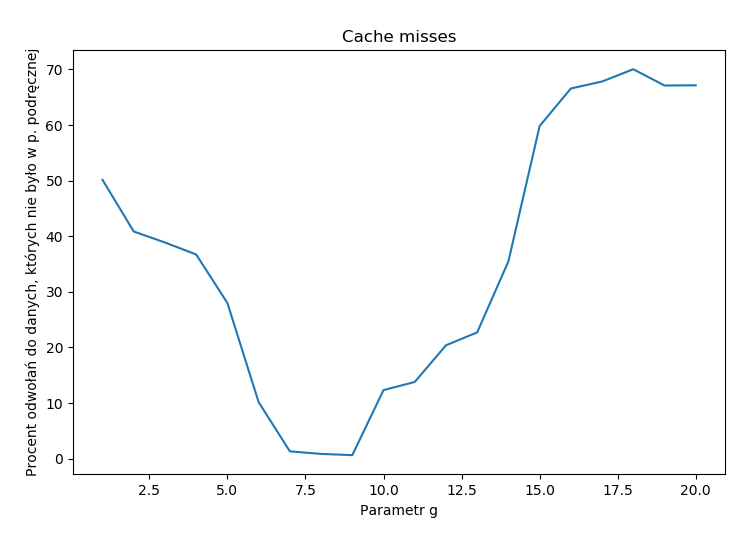
\includegraphics[width=\textwidth]{bench_1.png}
		\centering
		\caption{Wykresy liczby odczytów spoza pamięci podręcznej.}
		\label{impl::b1}
	\end{subfigure}
	\begin{subfigure}{0.5\textwidth}
		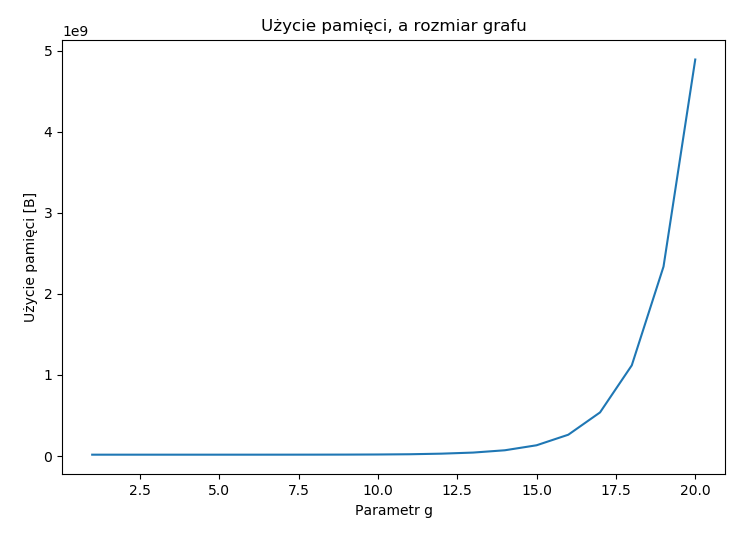
\includegraphics[width=\textwidth]{bench_2.png}
		\centering
		\caption{Wykresy zużycia pamięci przez $\mathbf{RiffleScrambler}$ w zależności od parametru $g$.}
		\label{impl::b2}
	\end{subfigure}
	\begin{subfigure}{0.5\textwidth}
		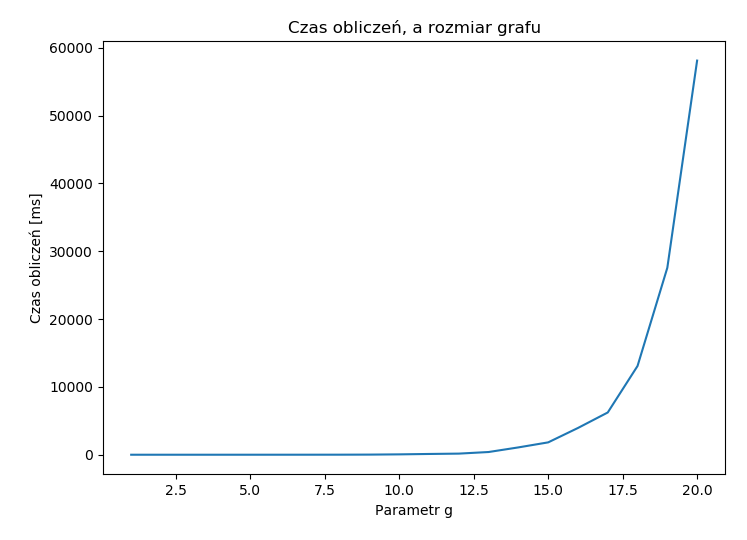
\includegraphics[width=\textwidth]{bench_3.png}
		\centering
		\caption{Wykres czasu obliczania $\mathbf{RiffleScrambler}$ w zależności od parametru $g$.}
		\label{impl::b3}
	\end{subfigure}
	\begin{subfigure}{0.5\textwidth}
		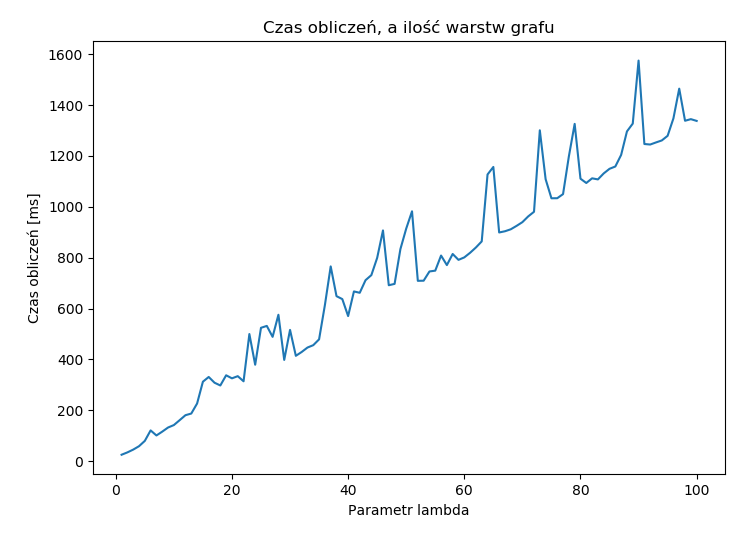
\includegraphics[width=\textwidth]{bench_4.png}
		\centering
		\caption{Wykres czasu obliczania $\mathbf{RiffleScrambler}$ w zależności od parametru $\lambda$.}
		\label{impl::b4}
	\end{subfigure}
		\begin{subfigure}{0.5\textwidth}
		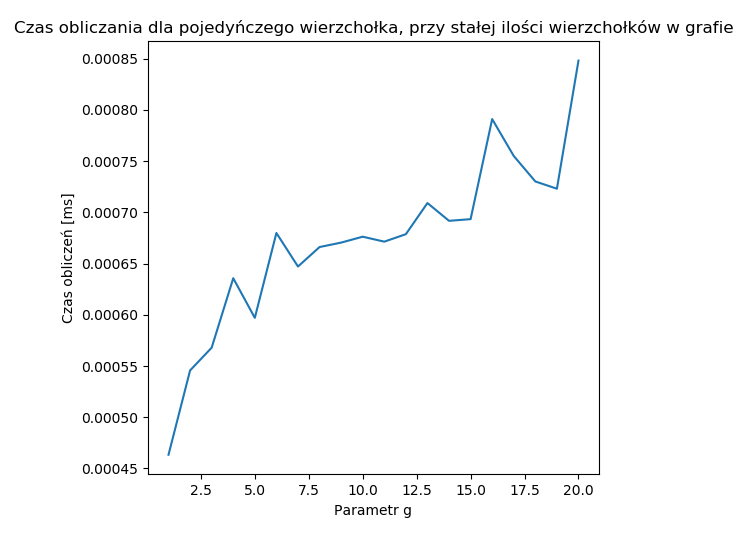
\includegraphics[width=\textwidth]{bench_5.png}
		\centering
		\caption{Wykres czasu obliczania $\mathbf{RiffleScrambler}$ w zależności od parametru $g$ dla stałej liczby wierzchołków w grafie.}
		\label{impl::b5}
	\end{subfigure}
	\begin{subfigure}{0.5\textwidth}
		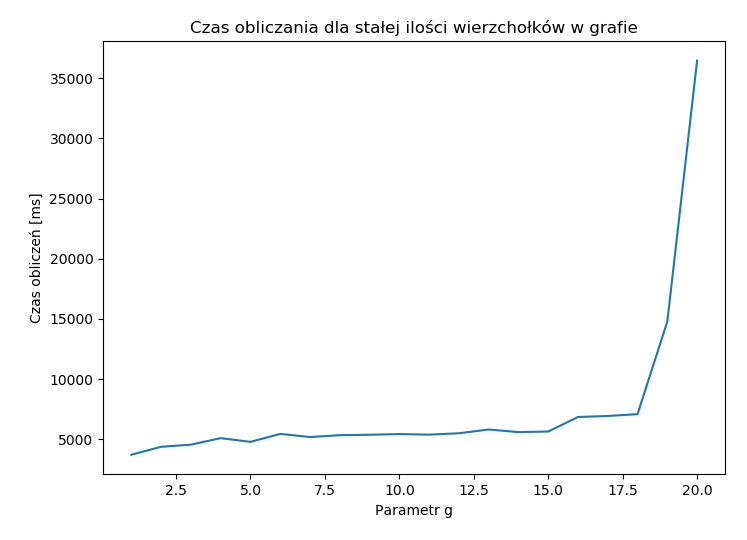
\includegraphics[width=\textwidth]{bench_6.png}
		\centering
		\caption{Średni czas obliczania jednego wierzchołka w zależności od parametru $g$ dla stałej liczby wierzchołków w grafie.}
		\label{impl::b6}
	\end{subfigure}

\end{figure}

\section{$\mathbf{RiffleScrambler}$ z wiersza poleceń}
Do implementacji dołączony został też program \texttt{rs} uruchamiany z wiersza poleceń umożliwiający testowanie działania funkcji $\mathbf{RiffleScrambler}$ w łatwy sposób.
Aby wyświetlić instrukcje, jak używać tego programu należy wykonać polecenie \texttt{./rs -h} lub \texttt{./rs --help}.

\begin{lstlisting}
$ ./rs --help             
Password hashing memory-hard function
Usage:
RiffleScrambler  Password is read from stdin [OPTION...] [optional args]

-s, --salt arg   Salt for the given password
-w, --width arg  Width of the graph (default: 12)
-d, --depth arg  Number of stacks of the graph (default: 2)
-f, --func arg   Internal hash function (default: sha256)
-h, --help       Print help
\end{lstlisting}

Program przyjmuje parametry do uruchomienia funkcji $\mathbf{RiffleScrambler}$ w argumentach wywołania, natomiast hasło przyjmuje na standardowe wejście, ponieważ większość wierszy poleceń zapisuje historię wywołań programów i hasło podane jako argument wywołania mogłoby zostać zapisane w postaci jawnej.

Przykład użycia programu do obliczenia funkcji dla hasła \texttt{password}, soli \texttt{somesalt}, parametru g \texttt{16}, parametru $\lambda$ \texttt{2} używając \texttt{sha256} jako funkcji wewnętrznej.
\begin{lstlisting}[language=bash]
$ echo -n "password" | ./rs somesalt -w 16 -d 2 -f sha224
Graph width:	16
Graph depth:	2
Hash:       	166c88a5edfba7228fbf49a4bcd4cb2f01cc5fcdc850bf78c317a5c8
Encoded:    	$g=16$d=2$s=c29tZXNhbHQ=$f=sha224$h=MTY2Yzg4YTVlZGZiYTcyMjhmYmY0(...)
\end{lstlisting}

\section{Przykład użycia}
Wysokopoziomowy interfejs umożliwia uwierzytelnianie w wygodny sposób.
Zaprezentowany zostanie przykład użycia biblioteki \texttt{riffle} w aplikacji internetowej
podłączonej do bazy danych SQL. Aplikacja ta pozwala na zakładanie kont dla nowych użytkowników, oraz po zalogowaniu się na konto przez użytkownika, udostępnia użytkownikowi pewne zasoby.
Biblioteka \texttt{riffle} zostanie wykorzystana przy tworzeniu nowego konta, w celu obliczenia wartości funkcji $\mathbf{RiffleScrambler}$ dla hasła użytkownika, którą można bezpiecznie trzymać w bazie danych oraz później podczas uwierzytelniania w celu weryfikacji poprawności hasła.


Tabela użytkowników w bazie danych została utworzona następująco.
\begin{minted}[linenos=true]{SQL}
CREATE TABLE Users (
UserID int,
Login varchar(255),
HahsEncoded varchar(255),
Name varchar(255),)
);
\end{minted}

\begin{minted}[mathescape]{C++}
// importowanie interfejsu z biblioteki
#include <riffle/riffle_scrambler.h>


/**
* Funkcja zapisująca użytkownika w bazie danych
* @param login Login użytkownika
* @param password Hasło użytkownika (w postaci jawnej)
* @param name Imie użytkownika
* @param address Adres użytkownika
*/
void create_account(const std::string &login, const std::string &password,
	const std::string &name, const std::string &address) {
	
	// stowrzenie połączenia do bazy danych SQL
	const auto database_adapter = get_sql_database_adapter();

	// generowana jest losowa sól
	const std::string salt = generate_random_salt();
	// hasło użytkownika jest hashowane dla podanych parametrów oraz soli
	const std::string hash_encoded = riffle_scrambler_encoded(12, 4, password, salt);

	// jeden, bezpieczny do przechowywania
	// zawierający informacje o paramertach, soli oraz hashu tekst
	database_adapter.add_user(login, hash_encoded, name, address);
}


/**
* Funkcja do autoryzacji użytkownika na podstawie podanego hasła
* sprawdza, czy podane hasło jest takie samo, jak hasło podane przy tworzeniu konta,
* które zapisane jest w bazie danych
* @param login Login użytkownika
* @param password Hasło podane przez użytkownika
* @return true, jeśli podane przez użytkownika hasło jest poprawne,
* false w przeciwnym przypadku
*/
bool is_password_valid(const std::string &login, const std::string &password) {
	// stowrzenie połączenia do bazy danych SQL
	const auto database_adapter = get_sql_database_adapter();

	// pobranie wiersza z danymi użytkownika z bazy danych
	const auto user = database_adapter.get_user_by_login(login);

	// sprawdzenie czy wynik funkcji riffle_scrambler dla podanego przez użytkownika hasła
	// zgadza się z poprawnym hasłem dla podanego loginu
	return riffle_scrambler_verify(user.hash_encoded, password);
}
\end{minted}

To, co zasługuje na docenienie podczas używania biblioteki \texttt{riffle}, to konieczność poświęcenia tylko jednej kolumny w tabeli, aby uzyskać możliwość uwierzytelniania użytkownika za pomocą hasła. Nie trzeba przechowywać soli, ani parametrów funkcji, ponieważ zawarte są one w zakodowanej wartości. Oznacza to, że można zmienić dowolne parametry funkcji używane podczas tworzenia nowych kont oraz uwierzytelniać użytkowników z hasłami zapisanymi wcześniej bez konieczności rozróżniania z jakimi parametrami jaki użytkownik zakładał konto.


